%!TEX root = ../../main.tex

\graphicspath{{../../figures/appendix/}}

\chapter{Simulations} \label{ch:appendix_simulation}

\newpage

\section{Spots and cluster simulations} \label{sec:appendix_simulations_spots}

\vfill

Figure~\ref{fig:spots_mosaic} is a sample of simulated images of spots.
We modulate the number of spots and the intensity of the noise for each image.

\vfill

\begin{figure}[h]
    \centering
    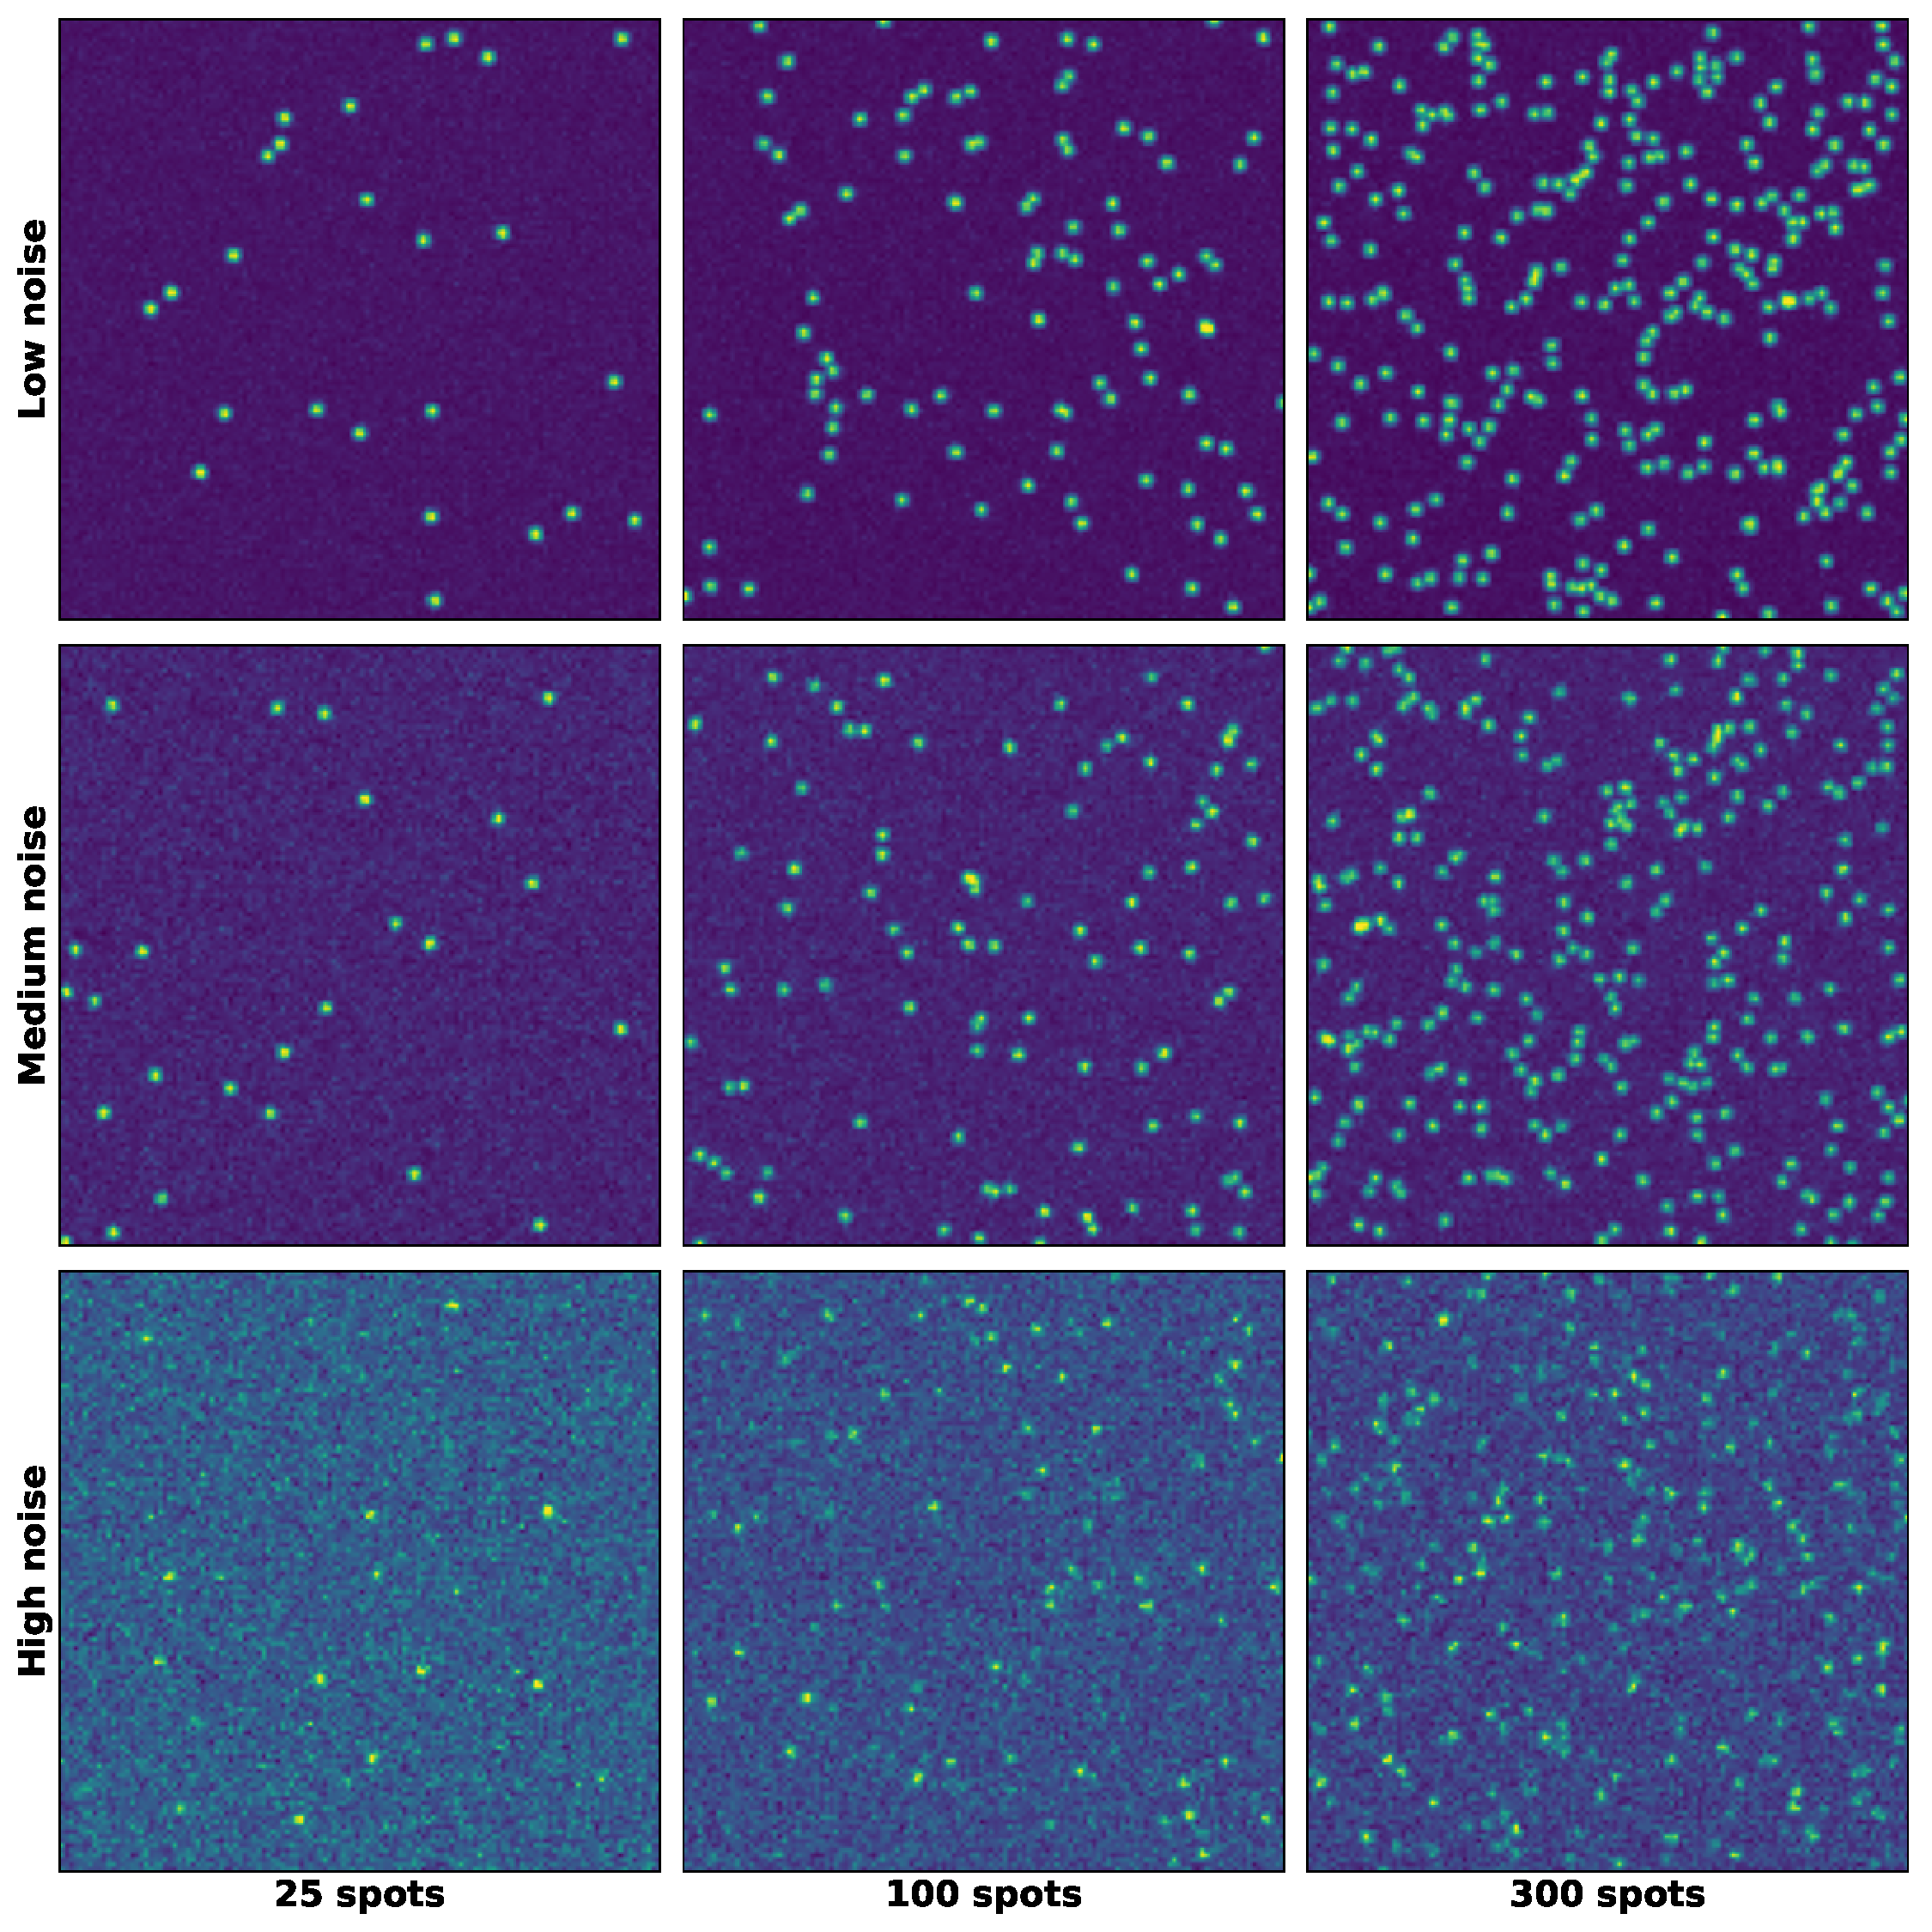
\includegraphics[width=\textwidth]{figures/appendix/spots_mosaic}
    \caption{Simulations of spots under different noise regimes}
    \label{fig:spots_mosaic}
\end{figure}

\newpage

\null
\vfill

Figure~\ref{fig:cluster_mosaic} use the same logic but with an unique cluster of spots simulated in the center.
This time, we modulate the number of spots inside the cluster.

\vfill

\begin{figure}[h]
    \centering
    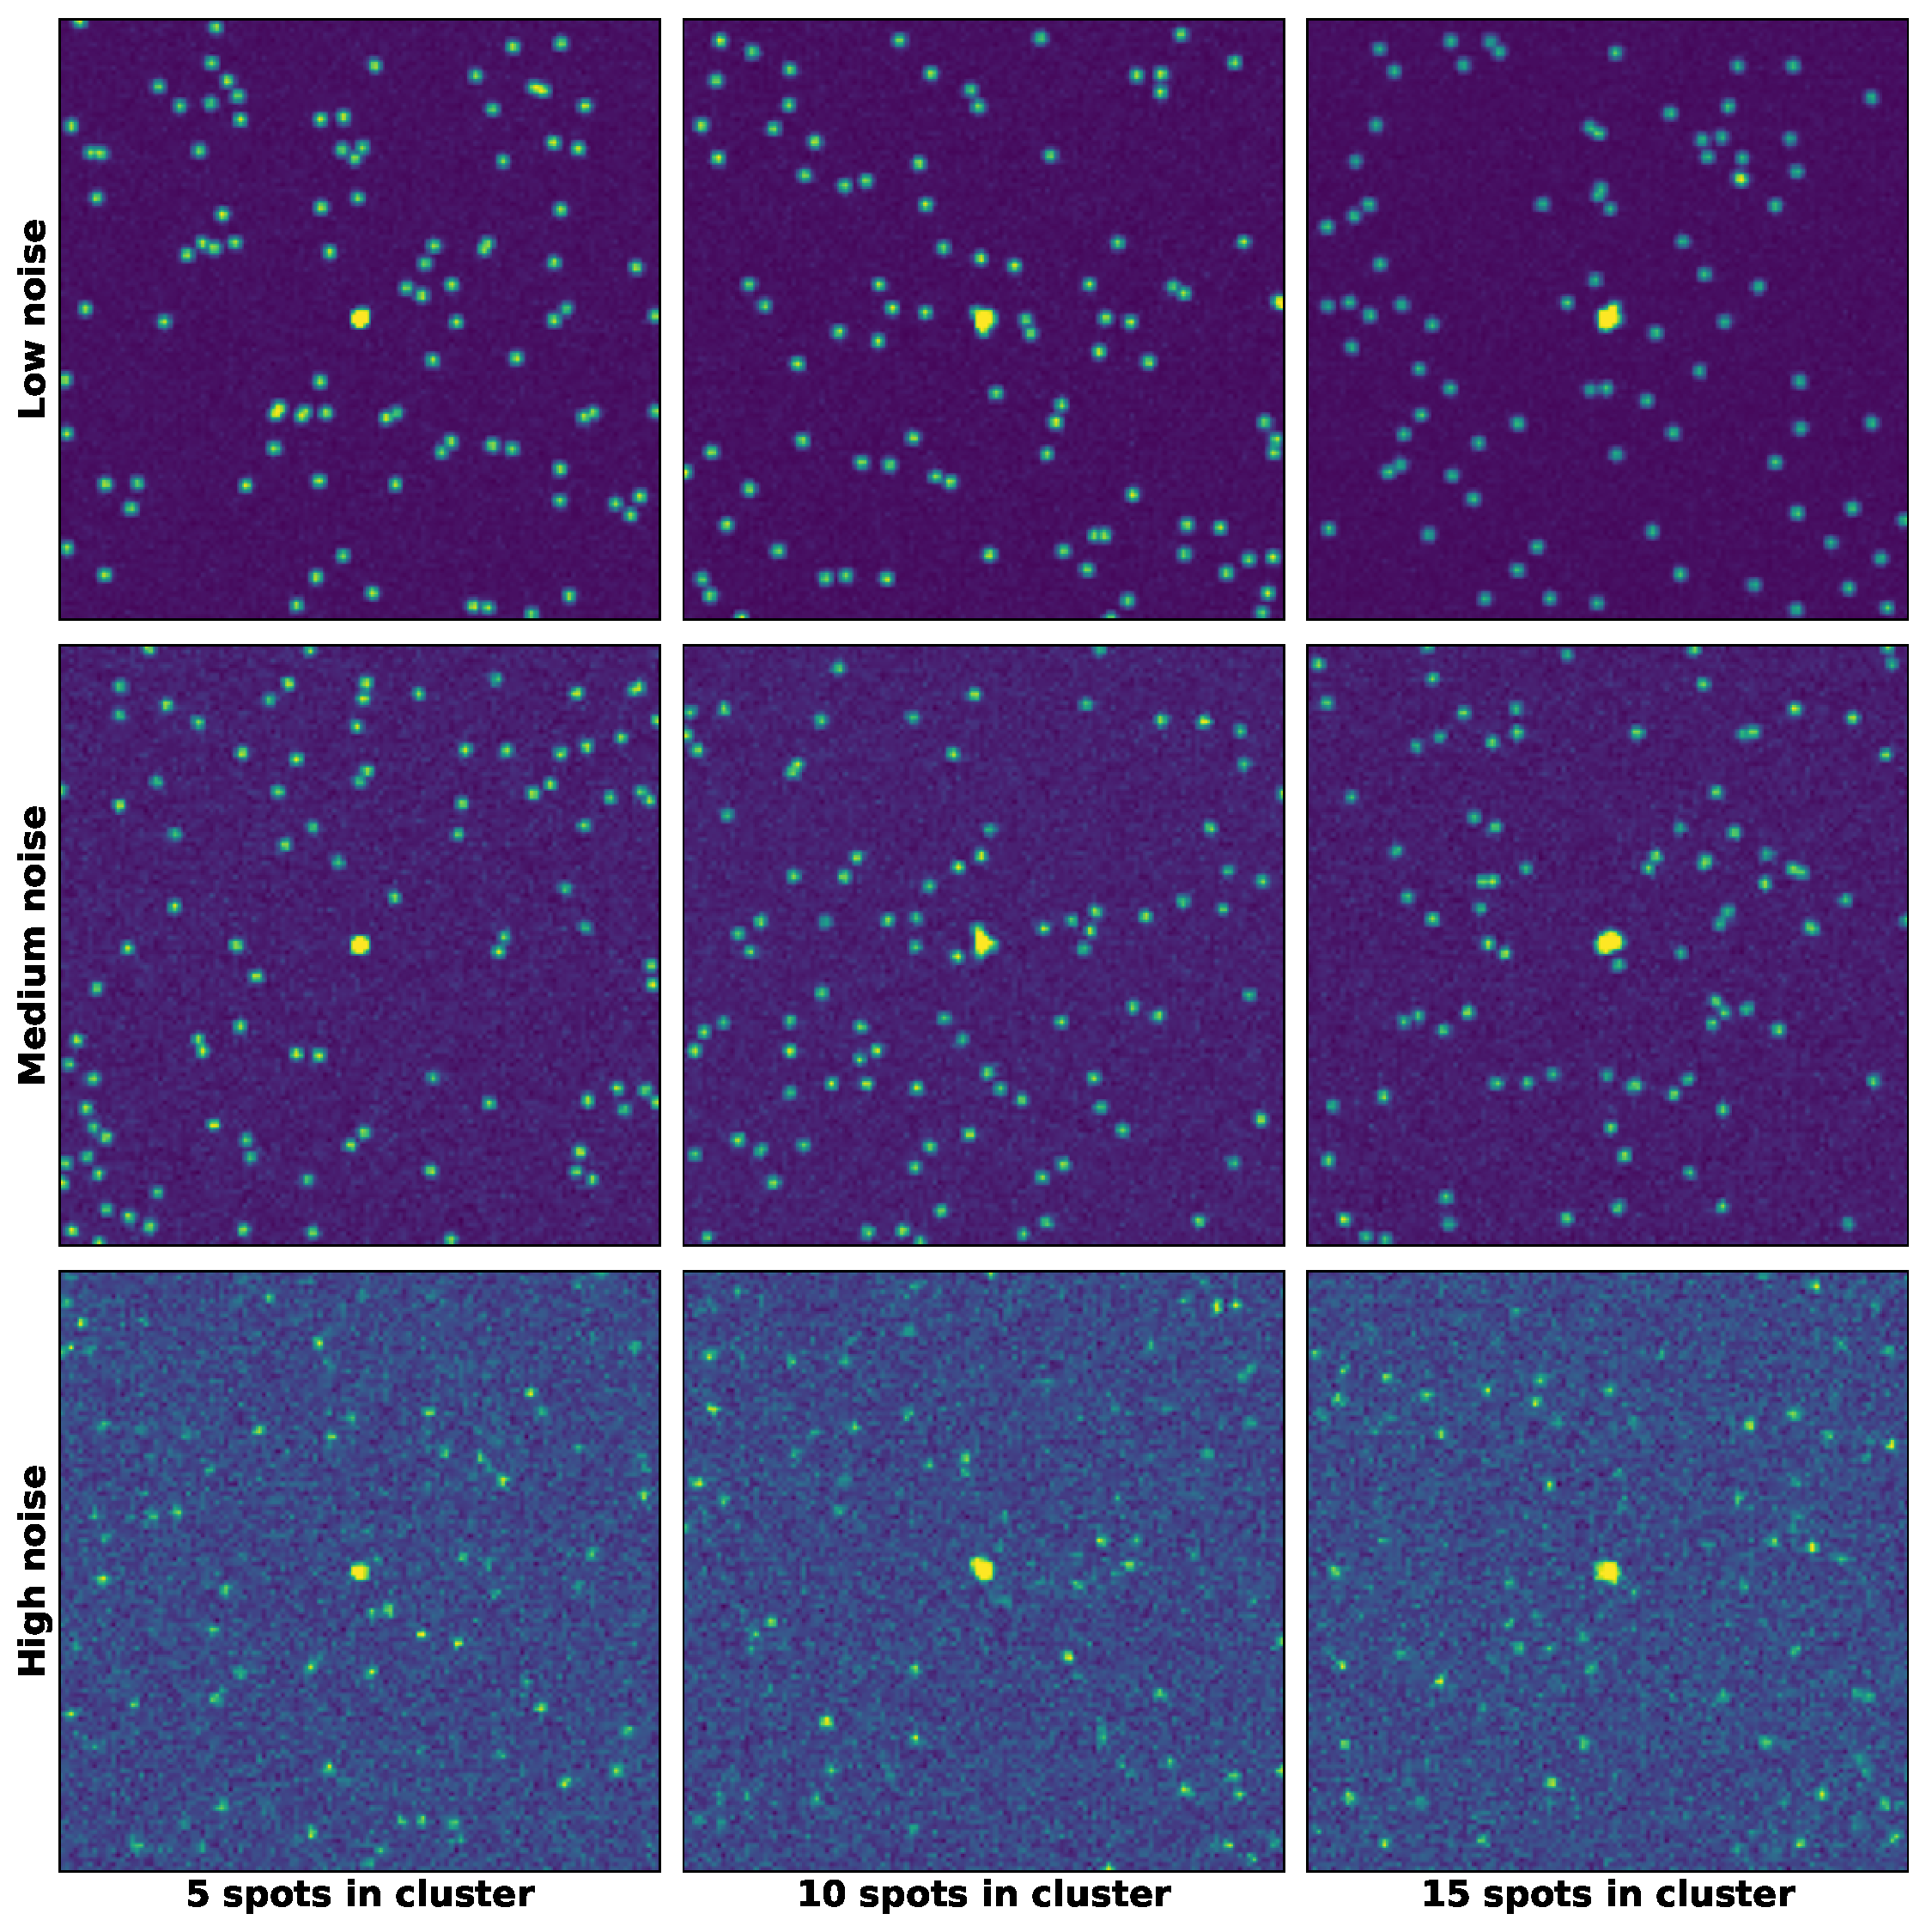
\includegraphics[width=\textwidth]{figures/appendix/cluster_mosaic}
    \caption{Simulations of cluster under different noise regimes}
    \label{fig:cluster_mosaic}
\end{figure}

\newpage

\section{Localization pattern simulations} \label{sec:appendix_simulations_pattern}
